\documentclass[tikz,border=8pt]{standalone}
% Shared look for every TikZ diagram. Load with \input{../../tools/tikz-style.tex}
\usepackage[T1]{fontenc}
\usepackage{lmodern}
\renewcommand{\sfdefault}{lmr}  % diagrams use the same serif as the text
\usetikzlibrary{arrows.meta, positioning, shapes.geometric, calc, fit, backgrounds}
\definecolor{cblue}{HTML}{4C78A8}
\definecolor{corange}{HTML}{F58518}
\definecolor{cgreen}{HTML}{54A24B}
\definecolor{cred}{HTML}{E45756}
\definecolor{cpurple}{HTML}{B279A2}
\definecolor{cgrey}{HTML}{6B6B6B}
\tikzset{
  every picture/.style={font=\sffamily, line width=1.2pt},
  box/.style={draw=#1, fill=#1!12, rounded corners=4pt, align=center, inner sep=7pt, minimum height=1.1cm},
  box/.default=cgrey,
  arrow/.style={-{Stealth[length=3mm]}, draw=cgrey, line width=1.4pt},
  title/.style={font=\sffamily\bfseries\Large},
  note/.style={font=\sffamily\small, text=cgrey, align=center},
}
\AtBeginDocument{\hyphenpenalty=10000 \exhyphenpenalty=10000}

\begin{document}
% Section 6: prediction with greedy decoding. The decoder's input at each step is its own previous output, so the
% wrong word "jao" at step 2 becomes the input of step 3. The toy output "soch jao lo" is the one named in section 6.
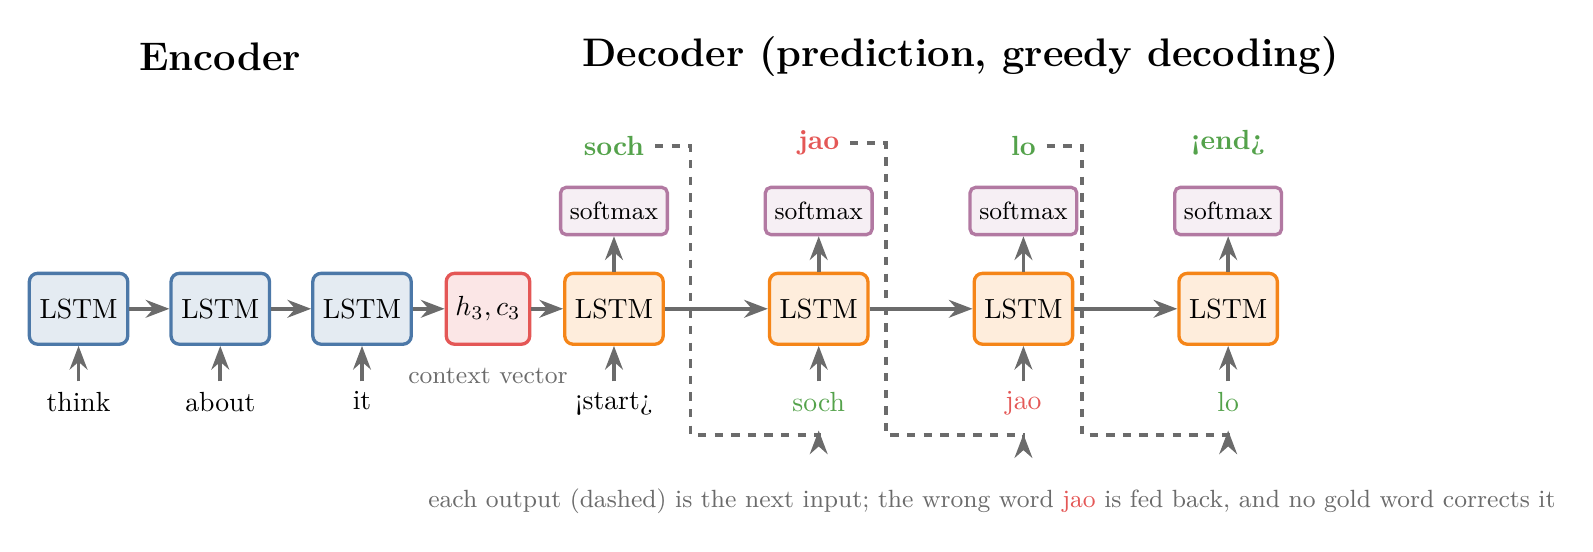
\begin{tikzpicture}[cell/.style={draw=#1, fill=#1!15, minimum width=1.25cm, minimum height=0.9cm, rounded corners=3pt, font=\sffamily},
  word/.style={font=\sffamily}, sm/.style={draw=cpurple, fill=cpurple!12, minimum width=1.25cm, minimum height=0.6cm, rounded corners=2pt, font=\sffamily\small}]
  \node[title] at (2.6, 3.2) {Encoder};
  \node[title] at (12.0, 3.2) {Decoder (prediction, greedy decoding)};
  \foreach \w [count=\i] in {think, about, it} {
    \node[cell=cblue] (e\i) at (1.8*\i - 1.0, 0) {LSTM};
    \node[word, below=0.45cm of e\i] (x\i) {\w};
    \draw[arrow] (x\i) -- (e\i);
  }
  \draw[arrow] (e1) -- (e2); \draw[arrow] (e2) -- (e3);
  \node[draw=cred, fill=cred!15, rounded corners=3pt, minimum height=0.9cm, font=\sffamily] (c) at (6.0, 0) {$h_3, c_3$};
  \node[note, below=0.15cm of c] {context vector};
  \draw[arrow] (e3) -- (c);
  \foreach \w/\p/\col [count=\i] in {{<start>}/soch/cgreen, soch/jao/cred, jao/lo/cgreen, lo/{<end>}/cgreen} {
    \node[cell=corange] (d\i) at (5.0 + 2.6*\i, 0) {LSTM};
    \node[sm, above=0.45cm of d\i] (s\i) {softmax};
    \draw[arrow] (d\i) -- (s\i);
    \node[word, above=0.25cm of s\i, text=\col] (p\i) {\textbf{\p}};
  }
  \foreach \w/\col [count=\i] in {{<start>}/black, soch/cgreen, jao/cred, lo/cgreen} {
    \node[word, below=0.45cm of d\i, text=\col] (y\i) {\w};
    \draw[arrow] (y\i) -- (d\i);
  }
  \foreach \i/\j in {1/2, 2/3, 3/4} {
    \draw[arrow, draw=cgrey, dashed, shorten >=3pt] (p\i.east) -- ++(0.45, 0) coordinate (k\i) -- (k\i |- 0, -1.6) -| (y\j.south);
  }
  \draw[arrow] (c) -- (d1); \draw[arrow] (d1) -- (d2); \draw[arrow] (d2) -- (d3); \draw[arrow] (d3) -- (d4);
  \node[note] at (12.4, -2.45) {each output (dashed) is the next input; the wrong word \textcolor{cred}{jao} is fed back, and no gold word corrects it};
\end{tikzpicture}
\end{document}
